% =============================================================================
% 00-abertura.tex - PARTE 0, abertura. Frames 01 a 03.
% =============================================================================

% ----------------------------------------------------------------- frame 01 --
% Capa. Unica excecao declarada de composicao: a ilustracao sangra de borda a
% borda e o texto ocupa a faixa central, que na arte e papel limpo. Os quatro
% cantos trazem, em sentido horario a partir do alto e a esquerda, o sofrimento
% isolado, o cuidado clinico, a rede que acolhe e o contato que se oferece, que
% e a propria cadeia da aula.
\begin{frame}[plain]
\CRar{0}
\begin{tikzpicture}[remember picture, overlay]
  \node[anchor=center, inner sep=0] at (current page.center) {%
    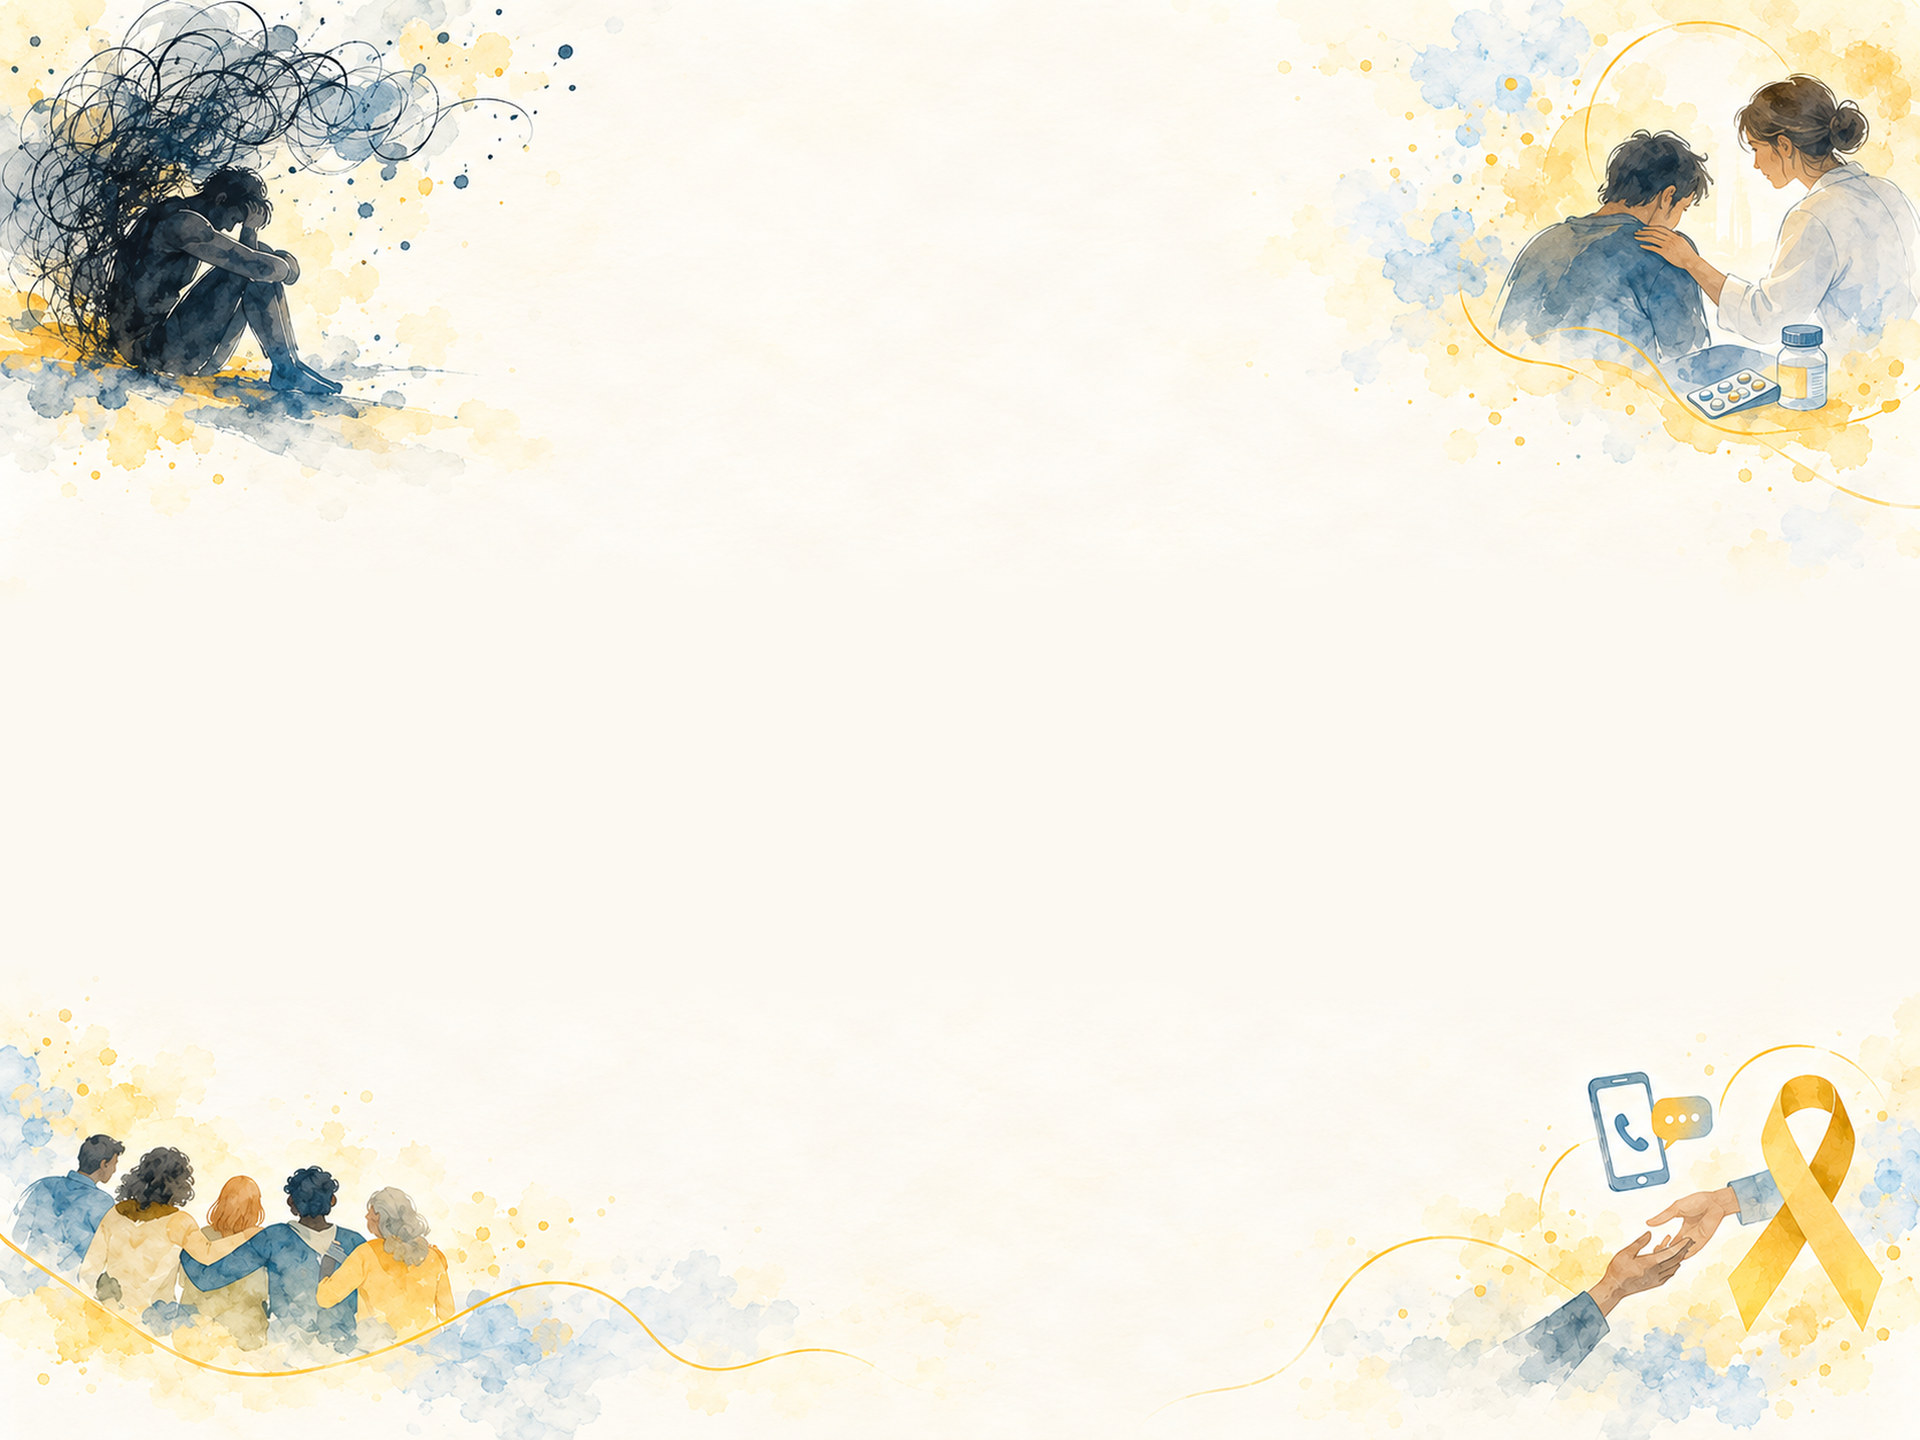
\includegraphics[width=\paperwidth, height=\paperheight]{ilustracoes/CAPA.jpg}};

  \node[anchor=center, align=center] at ($(current page.center)+(0,0.55cm)$) {%
    \begin{minipage}{8.2cm}\centering
      {\sffamily\bfseries\scriptsize\color{campobordo}%
       ATIVIDADE TE\'ORICO-PR\'ATICA}\\[0.30cm]
      {\sffamily\bfseries\LARGE\color{campoazul}Risco de suic\'idio}\\[0.14cm]
      {\sffamily\large\color{campoazul!75!black}avalia\c{c}\~ao e conduta}\\[0.34cm]
      {\color{campoamarelo!85!black}\rule{4.6cm}{1.6pt}}\\[0.30cm]
      {\sffamily\small\color{campografite}M\'odulo E3M40\\[0.05cm]
       Funcionalidade III, Cogni\c{c}\~ao e Humor}
    \end{minipage}};

  \node[anchor=south, align=center] at ($(current page.south)+(0,1.02cm)$) {%
    \begin{minipage}{7.0cm}\centering
      {\sffamily\footnotesize\color{campoazul!85!black}%
       \textbf{Prof. Jo\~ao Frederico Musial}}\\[0.06cm]
      {\sffamily\footnotesize\color{campografite}%
       Medicina \textbar{} Campo Real \textbar{} 2026}
    \end{minipage}};
\end{tikzpicture}
\end{frame}

% ----------------------------------------------------------------- frame 02 --
% Aviso de conteudo. Sobrio, sem dramatizacao, com saida garantida.
\begin{frame}{\ftit{\faHandHoldingHeart}{Antes de come\c{c}armos}}
\CRar{6}
\begin{caixaavaliar}{O que vamos discutir}
Esta aula trata de suic\'idio de forma direta, com falas de pacientes e com
decis\~oes cl\'inicas reais. N\~ao haver\'a imagem de m\'etodo, de cena nem de
les\~ao.
\end{caixaavaliar}

\CRvg
\begin{caixaproteger}{Voc\^e pode sair}
Se em algum momento voc\^e precisar se afastar, saia da sala. N\~ao \'e preciso
justificar, e isso n\~ao ser\'a registrado de nenhuma forma. Voltar depois
tamb\'em est\'a certo.
\end{caixaproteger}

\CRvg
\begin{center}
\begin{tikzpicture}
  \node[musialGreen, text width=9.2cm, font=\small] {%
    \faPhoneVolume~~\textbf{CVV 188}, liga\c{c}\~ao gratuita, 24 horas\\[2pt]
    \footnotesize O apoio ao estudante do Campo Real est\'a dispon\'ivel depois
    da aula. O docente tamb\'em est\'a.};
\end{tikzpicture}
\end{center}
\end{frame}

% ----------------------------------------------------------------- frame 03 --
% A pergunta da aula e a tese em duas linhas.
\begin{frame}{\ftit{\faQuestion}{A pergunta desta aula}}
\CRar{2.5}
\begin{center}
\begin{tikzpicture}
  \node[musialBlue, text width=9.0cm, font=\small, inner ysep=7pt] (p) {%
    \sffamily\bfseries \'E poss\'ivel construir seguran\c{c}a suficiente fora de
    um ambiente protegido neste momento?};
\end{tikzpicture}
\end{center}

\CRvg
\begin{caixaavaliar}{A tese}
O risco suicida \'e \avaliar{formula\c{c}\~ao cl\'inica din\^amica}, constru\'ida
pela intera\c{c}\~ao entre vulnerabilidades basais e modificadores proximais, e
n\~ao se reduz a escore nem a categoria. A conduta deve produzir
\proteger{seguran\c{c}a agora} e \proteger{continuidade depois}.
\end{caixaavaliar}

\CRvg
\begin{center}
\begin{tikzpicture}[node distance=0.20cm]
  \node[crnode={campoazul}{1.42cm}, font=\scriptsize, inner xsep=4pt] (a) {avaliar};
  \node[crnode={campoazul}{1.42cm}, font=\scriptsize, inner xsep=4pt, right=of a] (b) {formular};
  \node[crnode={campobordo}{1.42cm}, font=\scriptsize, inner xsep=4pt, right=of b] (c) {decidir};
  \node[crnode={campoverde}{1.70cm}, font=\scriptsize, inner xsep=4pt, right=of c] (d) {construir\\seguran\c{c}a};
  \node[crnode={campoverde}{1.70cm}, font=\scriptsize, inner xsep=4pt, right=of d] (e) {garantir\\continuidade};
  \draw[crseta=campoazul]  (a.east) -- (b.west);
  \draw[crseta=campoazul]  (b.east) -- (c.west);
  \draw[crseta=campobordo] (c.east) -- (d.west);
  \draw[crseta=campoverde] (d.east) -- (e.west);
\end{tikzpicture}
\end{center}

\mensagem{Ao final: o que, neste paciente, muda o que voc\^e far\'a nos
pr\'oximos 30 minutos?}
\end{frame}
